\documentclass{report}
\usepackage[utf8]{inputenc}
\usepackage[top=2.5cm, left=2.3cm, right=2.7cm, bottom=3.0cm]{geometry}
\usepackage{accents}
%\usepackage{amsmath}
\usepackage{float}
\usepackage{hyperref}
\usepackage{pdfpages}
\usepackage{sectsty}
\usepackage{titlesec}
\usepackage{listings}
\usepackage{graphicx}
\graphicspath{ {./images/} }

\titleformat{\chapter}{\normalfont\huge}{\thechapter.}{20pt}{\huge\it}
\newcommand{\ubar}[1]{\underaccent{\bar}{#1}}
\newcommand{\e}[1]{\cdot10^{#1}}


\title{\huge Report 2 \\ \Huge System Programming}
\author{\huge Baran Hasan Bozduman\\ \huge 171044036}
\date{\today}
\begin{document}
\maketitle
{\huge \textbf{Problem Definition} \\}

{\large The problem was implementing a calculation program with child processes each child will be responsible for different calculations) \\}

{\huge \textbf{Design Decision} \\}

{\large I calculated Lagrange by using online resources one of them is gfg other one was a javascript code so I struggle it into c language and i can find all values correctly.  \\}
{\large For the synchronization I tried to implement a flag similar structure firstly it creates children of the parent processes then execute it for first round then it waits signal from his parent and after parent say them you can continue it starts to run second round and make the calculations for rest of them. Parent and children send signals to each other to determine when they should continue or when they should stop but  I implement it but it is not working correctly for second round it stops working somehow(probably because of sigint the child can not take the some signals I could not merge because of other lessons) and it waits for the signal to continue other parts so i send them separately  \\}
\newline
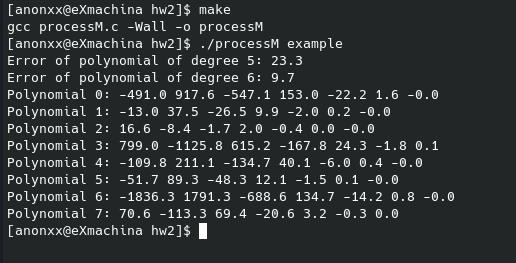
\includegraphics{images/lag.png}
\newline
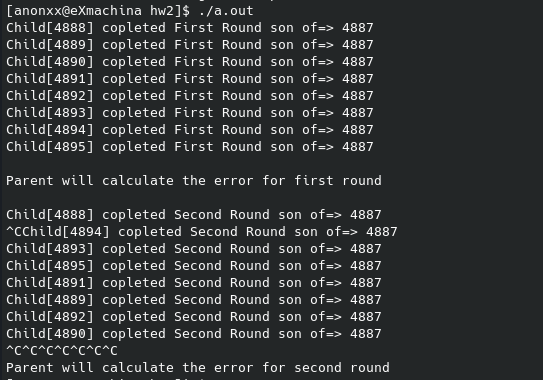
\includegraphics{images/sig.png}

{\huge \textbf{The Requirements I have achieved} \\}
 {\large I tried the rules below and they worked properly on my computer}
\begin{enumerate}
    \item {\large No compilation error }
    \item {\large No compilation warning}
    \item {\large \check{Make file} }
    \item {\large \check{Report in Latex format}}
    \item {\large Printed usage information in case of missing or invalid argument}
    \item {\large Program did not crashed}
    \item {\large No memory leaks}
    \item {\large Submitted on time}
    \item {\large Informed user in case of system errors}
    \item {\large It opens file and creates children in second file!}
    
\end{enumerate}

{\huge \textbf{The Requirements I have failed} \\}

{\large  For second round Synchronization is not completed so I send it in another file \\}


\end{document}
